
\let\negmedspace\undefined
\let\negthickspace\undefined
\documentclass[journal,12pt,twocolumn]{IEEEtran}

\usepackage{cite}
\usepackage{amsmath,amssymb,amsfonts,amsthm}
\usepackage{algorithmic}
\usepackage{graphicx}
\usepackage{textcomp}
\usepackage{xcolor}
\usepackage{txfonts}
\usepackage{listings}
\usepackage{enumitem}
\usepackage{mathtools}
\usepackage{gensymb}
\usepackage[breaklinks=true]{hyperref}
\usepackage{tkz-euclide} % loads  TikZ and tkz-base
\usepackage{listings}

\DeclareMathOperator*{\Res}{Res}
%\renewcommand{\baselinestretch}{2}
\renewcommand\thesection{\arabic{section}}
\renewcommand\thesubsection{\thesection.\arabic{subsection}}
\renewcommand\thesubsubsection{\thesubsection.\arabic{subsubsection}}

\renewcommand\thesectiondis{\arabic{section}}
\renewcommand\thesubsectiondis{\thesectiondis.\arabic{subsection}}
\renewcommand\thesubsubsectiondis{\thesubsectiondis.\arabic{subsubsection}}

% correct bad hyphenation here
\hyphenation{op-tical net-works semi-conduc-tor}
\def\inputGnumericTable{}                                 %%

\lstset{
	%language=C,
	frame=single, 
	breaklines=true,
	columns=fullflexible
}

\newcommand{\define}{\stackrel{\triangle}{=}}
\newcommand{\permcomb}[4][0mu]{{{}^{#3}\mkern#1#2_{#4}}}
\newcommand{\comb}[1][-1mu]{\permcomb[#1]{C}}

\begin{document}
	%
	
	
	\newtheorem{theorem}{Theorem}[section]
	\newtheorem{problem}{Problem}
	\newtheorem{proposition}{Proposition}[section]
	\newtheorem{lemma}{Lemma}[section]
	\newtheorem{corollary}[theorem]{Corollary}
	\newtheorem{example}{Example}[section]
	\newtheorem{definition}[problem]{Definition}
	
	\newcommand{\BEQA}{\begin{eqnarray}}
		\newcommand{\EEQA}{\end{eqnarray}}
	%	\newcommand{\define}{\stackrel{\triangle}{=}}
	
	\bibliographystyle{IEEEtran}
	%\bibliographystyle{ieeetr}
	
	
	\providecommand{\mbf}{\mathbf}
	\providecommand{\pr}[1]{\ensuremath{\Pr\left(#1\right)}}
	\providecommand{\qfunc}[1]{\ensuremath{Q\left(#1\right)}}
	\providecommand{\sbrak}[1]{\ensuremath{{}\left[#1\right]}}
	\providecommand{\lsbrak}[1]{\ensuremath{{}\left[#1\right.}}
	\providecommand{\rsbrak}[1]{\ensuremath{{}\left.#1\right]}}
	\providecommand{\brak}[1]{\ensuremath{\left(#1\right)}}
	\providecommand{\lbrak}[1]{\ensuremath{\left(#1\right.}}
	\providecommand{\rbrak}[1]{\ensuremath{\left.#1\right)}}
	\providecommand{\cbrak}[1]{\ensuremath{\left\{#1\right\}}}
	\providecommand{\lcbrak}[1]{\ensuremath{\left\{#1\right.}}
	\providecommand{\rcbrak}[1]{\ensuremath{\left.#1\right\}}}
	\theoremstyle{remark}
	\newtheorem{rem}{Remark}
	\newcommand{\sgn}{\mathop{\mathrm{sgn}}}
	\providecommand{\abs}[1]{\left\vert#1\right\vert}
	\providecommand{\res}[1]{\Res\displaylimits_{#1}} 
	\providecommand{\norm}[1]{\left\lVert#1\right\rVert}
	%\providecommand{\norm}[1]{\lVert#1\rVert}
	\providecommand{\mtx}[1]{\mathbf{#1}}
	\providecommand{\mean}[1]{E\left[ #1 \right]}
	\providecommand{\fourier}{\overset{\mathcal{F}}{ \rightleftharpoons}}
	%\providecommand{\hilbert}{\overset{\mathcal{H}}{ \rightleftharpoons}}
	\providecommand{\system}{\overset{\mathcal{H}}{ \longleftrightarrow}}
	%\newcommand{\solution}[2]{\textbf{Solution:}{#1}}
	\newcommand{\solution}{\noindent \textbf{Solution: }}
	\newcommand{\cosec}{\,\text{cosec}\,}
	\providecommand{\dec}[2]{\ensuremath{\overset{#1}{\underset{#2}{\gtrless}}}}
	\newcommand{\myvec}[1]{\ensuremath{\begin{pmatrix}#1\end{pmatrix}}}
	\newcommand{\mydet}[1]{\ensuremath{\begin{vmatrix}#1\end{vmatrix}}}
	
	\let\vec\mathbf
	
		
		\vspace{3cm}
		
		\title{Random Number Generator}
        \author{Gholap Siddhesh Ashok\\AI22BTECH11007}
	\maketitle	

\newpage



\bigskip

\renewcommand{\thefigure}{\theenumi}
\renewcommand{\thetable}{\theenumi}




\section*{\textbf{Components used}}
\begin{table}[h] % Place the table here (h stands for "here")
    \centering % Center the table horizontally
    \caption{components used} % Table caption
    \label{tab:tablelabel} % Table label for referencing
    \begin{tabular}{|c|c|c|} % Table columns and alignment
        \hline % Horizontal line
        \textbf{Component} & \textbf{Value} & \textbf{Quantity} \\ % Table header row
        \hline % Horizontal line
        Breadboard &  & 1 \\ % Table content row 1
        \hline
        Seven segment display & Common Anode & 1\\ % Table content row 2
        \hline
        Decoder & 7447 & 1\\
        \hline
        Flip Flop & 7474 & 2\\
        \hline
        X-OR Gate & 7486 & 1\\
        \hline
        555 IC & & 1\\
        \hline
        Resistor & 1K\ohm & 1\\
        \hline
        Capacitor & 100nF & 1\\
        \hline
        Capacitor & 10nF & 1\\
        \hline
        Jumper Wires & & \\
        \hline
    \end{tabular}
\end{table}



\section*{\textbf{Procedure}}
\begin{enumerate}
	\item We connected the 555 timer circuit according to the figure 
	
	
	\item Then we connected Clock output of 555 timer circuit to the clock signal of D-Flip flops
	
	\item Now we make the circuit for shift registers using a 4 D-Flip flops (using two 7474 IC's)
	

	\item Then we connected XOR gate (7486 IC) according to the figure  
	

	\item then we connected the decoder (7447 IC) and connected its A,B,C,D with $Q_0$,$Q_1$,$Q_2$,$Q_3$ respectively as per the figure 
	
		
	\item Then we connected The seven segmented display and then connected it with the dceoder (7447 IC) according to the table and the figure 

	\item We connected all the independent parts with each other and then connected the power source
	
	
\section*{Output} 
	Random numbers were displayed on the digital screen in a certain frequency.
	\begin{figure}[h]
		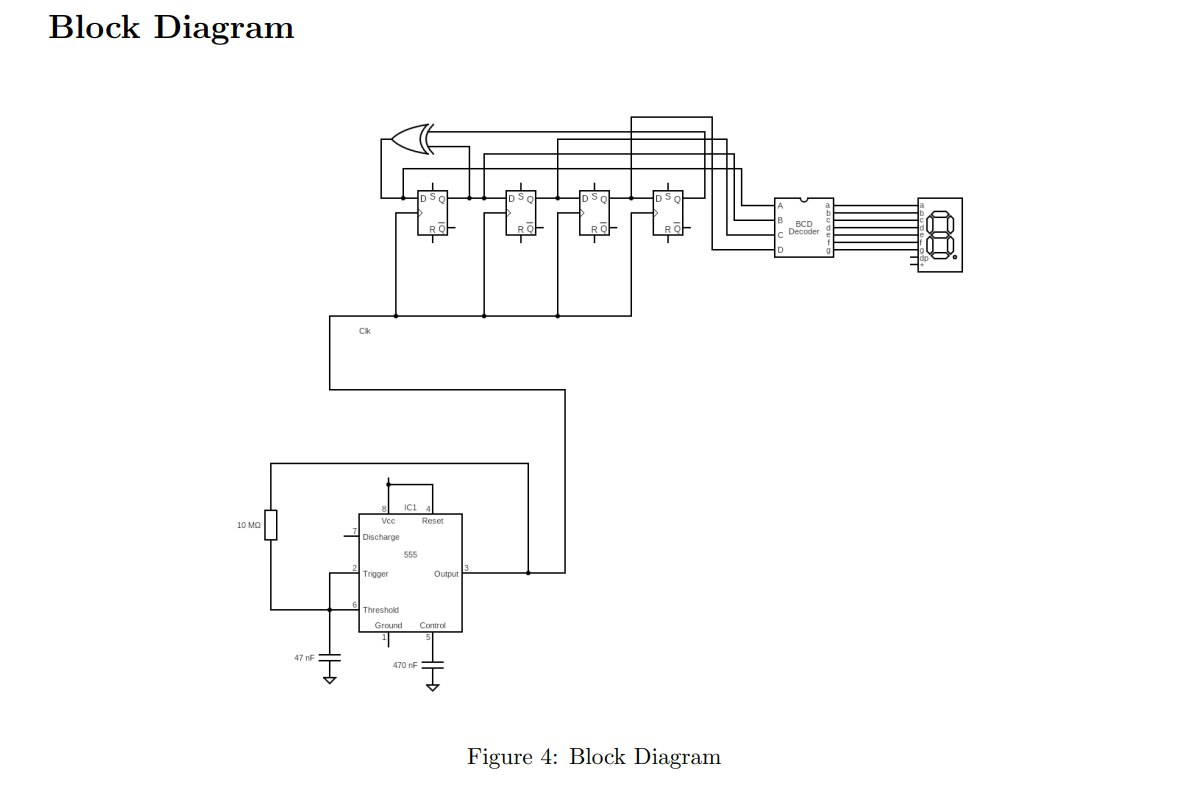
\includegraphics[width=\linewidth]{s1.jpg}
		\caption{output}
		\label{output}
	\end{figure}
	\begin{figure}[h]
		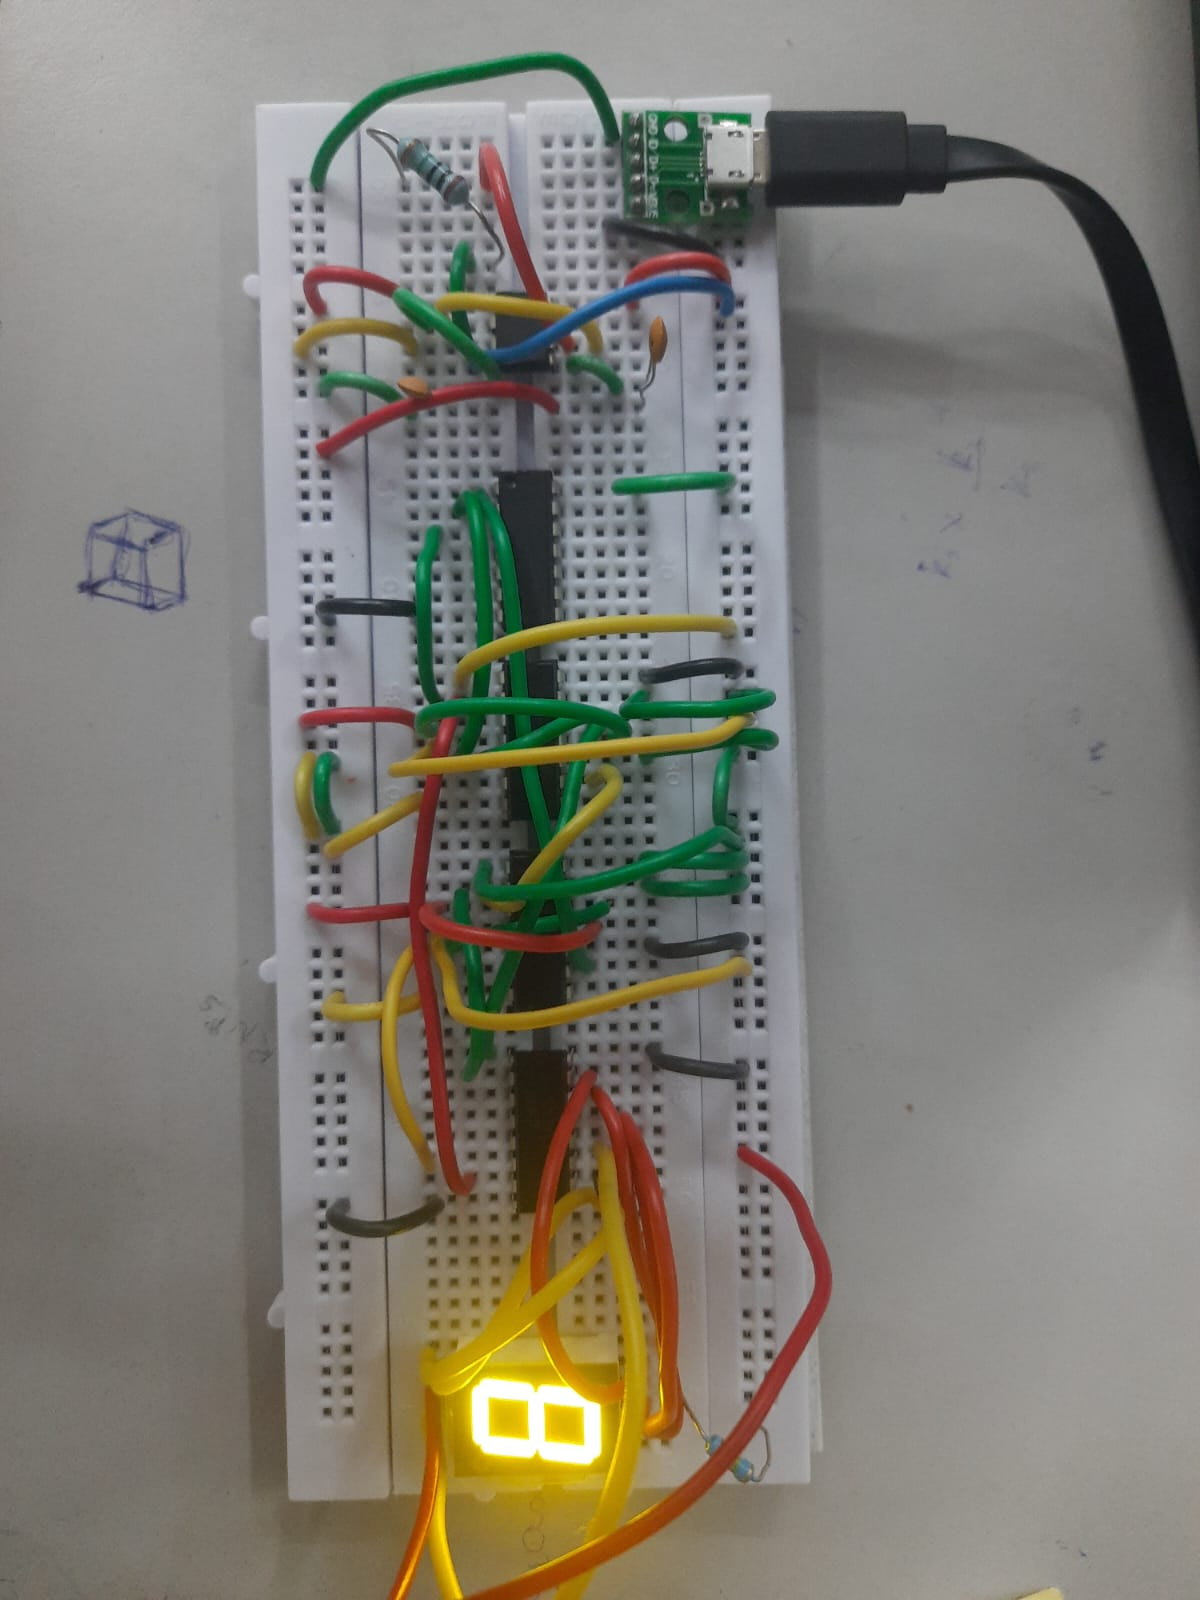
\includegraphics[width=\linewidth]{s2.jpeg}
		\caption{output}
		\label{output}
	\end{figure}
	\begin{figure}[h]
		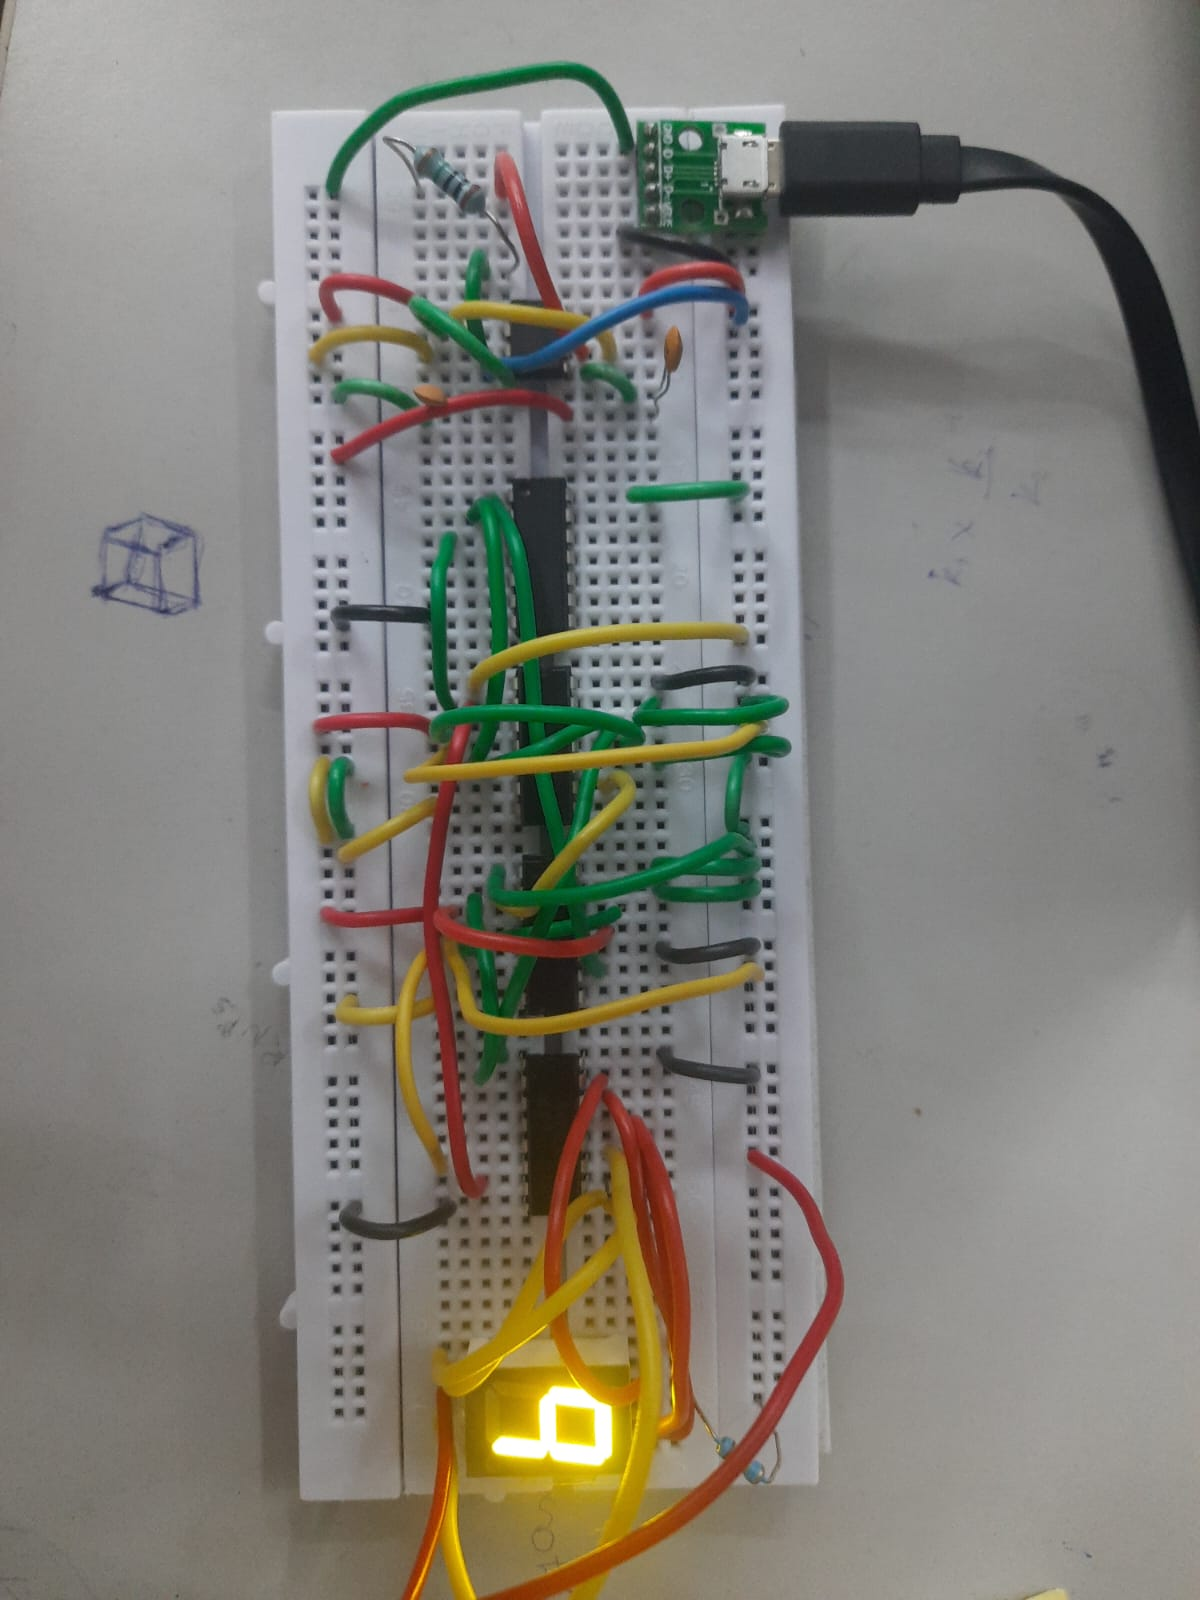
\includegraphics[width=\linewidth]{s3.jpeg}
		\caption{output}
		\label{output}
	\end{figure}
	
\end{enumerate}


\end{document}
